\documentclass[conference]{IEEEtran}
\IEEEoverridecommandlockouts
% The preceding line is only needed to identify funding in the first footnote. If that is unneeded, please comment it out.
\usepackage{cite}
\usepackage{amsmath,amssymb,amsfonts}
\usepackage{algorithmic}
\usepackage{graphicx}
\usepackage{textcomp}
\usepackage{xcolor}
\def\BibTeX{{\rm B\kern-.05em{\sc i\kern-.025em b}\kern-.08em
    T\kern-.1667em\lower.7ex\hbox{E}\kern-.125emX}}
\begin{document}

\title{Hydra Mini}

\author{\IEEEauthorblockN{1\textsuperscript{st} Tianze Wu}
\IEEEauthorblockA{
\textit{Insititute Of Computing Technology Chinese Academy Of Sciences}\\
{University of Chinese Academy of Sciences}\\
Beijing, China \\
wutianze@ict.ac.cn}
}
\maketitle

\begin{abstract}
Autonomous driving is a hot topic currently, many companies and research institutions have put a lot of effort into the topic. In this paper, we present xx car, an experimental research and education platform for autonomous driving. xx is based on Xilinx Pynq-Z2 and also uses the power of Deep learning Processing Unit(DPU) to accelerate the inference process and provides a simulator for training and testing in virtual environment. Our platform can help researchers and students who want to try autonomous driving or hardware accelerating build their own solutions and test it efficiently. We hope the xxx car meets three requirements: affordable, easy to understand and easy to use. 
\end{abstract}

%\begin{IEEEkeywords}
%Autonomous Driving, Machine Learning, Pynq-Z2, Field programmable gate arrays, Deep Learning Processing Unit
%\end{IEEEkeywords}

\section{Introduction}
With the development of AI technology, many work can be done by robot instead of human. Driving is one of these tasks and autonomous driving(AD) has become more and more popular these years. We can see from Google Trends of the keyword 'autonomous driving' from 2010 to 2019 in Fig.~\ref{st}, it's obvious that AD technology will be one of the hot topics of AI. The reason why this topic is so hot is that AD is not one single technology, but rather a highly complex system that consists of many sub-systems\cite{b1}, it's the area where any researcher can make contributions.

\begin{figure}[htbp]
\centerline{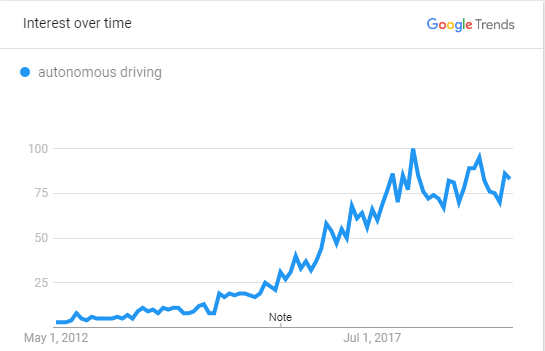
\includegraphics[width=0.5\textwidth]{search_result.PNG}}
\caption{Search Trend.}
\label{st}
\end{figure}

As a result, there will be more people trying to learn about AD technology. So a platform for AD researching and learning is badly needed. 

In the cloud computing domain, researchers usually want to own machines that have good computation performance. The data center based on virtualization technology\cite{b2} and distributed computing\cite{b3} nowadays usually has many powerful servers for data processing. Also, for AD tasks, accelerating the inference process through hardware is becoming more and more common and indispensable, it's the cornerstone of the development of AD and all the researchers and students should pay enough attention to it. However, when comes to systems in the car, we should care about not only the computing power but also the power consumption and cost. It's a pity that we can hardly find one product that can provide both enough computing power and hardware acceleration but remains affordable for most of the people.

To make everyone have the opportunity to participate in the research of AD, we propose xxx, an indoor experimental research and education platform for AD. The platform was first designed for the design competition of FPT 2019\cite{}, then we find the potential of this design and decide to make the project a common platform for researchers and students. As shown in Fig.~\ref{ov}, xxx is a powerful and flexible platform from hardware to software. It depends on three main components: mechanical component, control system and FPGA accelerator. We also provide a simulator using Unity3d\cite{b4} based on sdsandbox\cite{b5} that can make the users test their design more conveniently. All the resources on xxx are managed by Pynq-Z2\cite{b6} system which is based on Ubuntu 18.04\cite{b7}. 

Users can use the computing power in Pynq-Z2 includes both FPGA which can be used as a specialized hardware accelerator and an Arm 32-bit core ARM Cortex-A9\cite{b8} which is familiar to normal people. We believe that in the future the hardware acceleration will become an imperative for the modern cars to provide edge computing power, so it's necessary to embed FPGA which is flexible for researching in our platform. Users will find it easy to do research on multi-area of AD and develop their own algorithms and systems based on xxx.

\begin{figure}[htbp]
\centerline{\includegraphics[width=0.5\textwidth]{car.jpg}}
\caption{Overview of xxx Platform.}
\label{ov}
\end{figure}

\section{Related Work}

In this section, we summarize the related work and some other similar platforms.

\textbf{Research Platform for Autonomous Devices.} Yifan Wang et al. presented HydraOne\cite{b9}, HydraOne is an indoor robot-based platform, it has sufficient resources and components to conduct related experiments. It has three key characteristics: design modularization, resource extensibility and openness, as well as function isolation, which allows users to conduct various research and education experiments. Wei et al. presented the CMU autonomous driving research platform which is based on a Cadillac SRX\cite{b10}. This work focuses on vehicle engineering problems, including the actuation, power, and sensor systems on the vehicle. Matthew O’Kelly et al present F1/10\cite{b11}: an open-source, affordable, and high-performance 1/10 scale autonomous vehicle testbed. The F1/10 testbed carries a full suite of sensors, perception, planning, control, and networking software stacks that are similar to full scale solutions. 

\textbf{Hardware Acceleration Technology.} GPU\cite{b12} is now widely used by researchers to accelerate the training and inference process of AI. The training library is cuDNN\cite{b13} while the inference library is TensorRT\cite{b14}. cuDNN is a GPU-accelerated library of primitives for deep neural networks. It provides highly tuned implementations of routines arising frequently in DNN applications. TensorRT focuses specifically on running an already trained network quickly and efficiently on a GPU for the purpose of generating a result; also known as inferencing. The tensor processing unit was announced in May 2016 at Google I/O, when the company said that the TPU had already been used inside their data centers for over a year\cite{b15}. The chip has been specifically designed for Google's TensorFlow framework, a symbolic math library which is used for machine learning applications such as neural networks.\cite{b16} The Xilinx Deep Learning Processor Unit (DPU)\cite{b17} is a programmable engine optimized for convolutional neural networks. The unit includes a high performance scheduler module, a hybrid computing array module, an instruction fetch unit module, and a global memory pool module. The DPU uses a specialized instruction set, which allows for the efficient implementation of many convolutional neural network.

\section{Design and Implementation}
In this section, we introduce the design and implementation details of xxx and present main characteristics of the platform.

\subsection{Hardware Design}


\begin{figure}[htbp]
\centerline{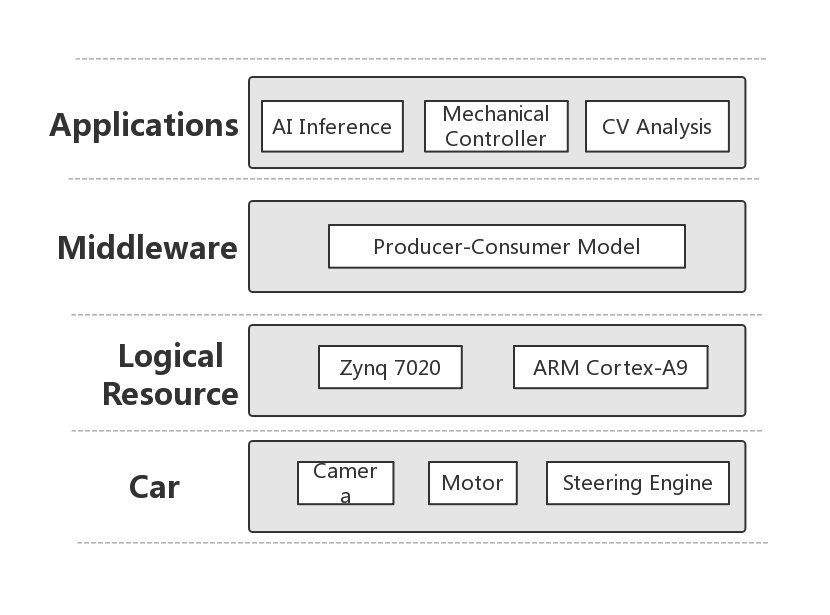
\includegraphics[width=0.5\textwidth]{sf.jpg}}
\caption{Hardware Design.}
\label{hd}
\end{figure}

\subsection{Software Design}
\textbf{Framework Overview.} The operating system on Pynq-Z2 is based on Ubuntu 18.04, so the users can easily install the libraries they need. The system on Pynq-Z2 also provides many jupyter notebook documents about how to fully utilize the hardware resources in Pynq-Z2. To make the control process more efficient and easier to extend, we implement a producer-consumer model\cite{b18} which is a classic design pattern in multi-process synchronization environment. The whole control system depends on three main components: mechanical controller, AI model inference and computer vision auxiliary analysis. The structure of the system is shown in Fig.~\ref{sf}. It's easy for users to add or remove component to or from the system. 

\begin{figure}[htbp]
\centerline{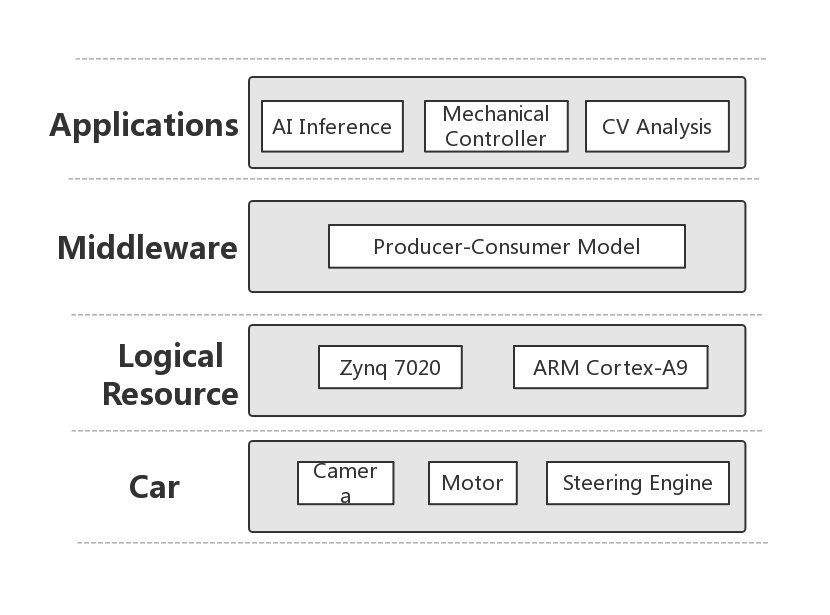
\includegraphics[width=0.5\textwidth]{sf.jpg}}
\caption{Software Framework.}
\label{sf}
\end{figure}

\textbf{Producer-Consumer model.} Many indoor AD driving platforms like HydraOne\cite{b9} and F1/10\cite{b11} use ROS\cite{b19} to manage the hardware and software resources nowadays because ROS can provide the car with an easy way to communicate with the server and many existing applications. However, to make a balance between the platform's cost and performance, we focuses mainly on some core functions in AD and the communication between car and server is not so important. Using ROS will bring unnecessary overhead to CPU. So a more streamlined and efficient method is used as the base of the control system. You can refer to Fig.~\ref{pcm} for an overview of this model.


\begin{figure}[htbp]
\centerline{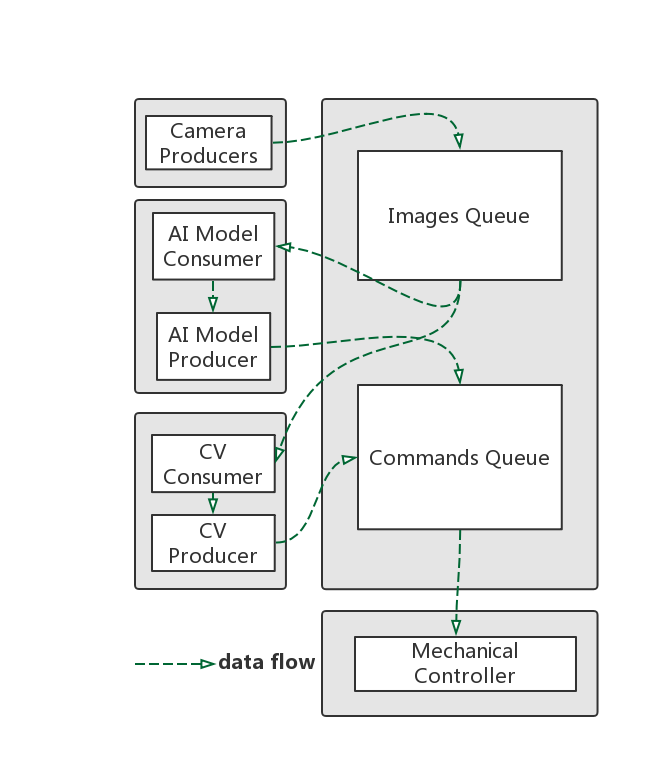
\includegraphics[width=0.5\textwidth]{pcm.jpg}}
\caption{Producer-Consumer Model.}
\label{pcm}
\end{figure}

The sensors like camera will play the role of producer while the decision makers like AI model and computer vision methods will be consumers. Each kind of data will be stored in a queue in memory. Different producer processes add the data they get to the specified queue and will be handled by consumers who cares about this kind of data. It's easy to add more producers or consumers and new kind of data. If one process want to handle or provide different kind of data, just read or write the related queue. The synchronism of the system is maintained by locks, each queue will have a lock.

The consumers who usually act as controller have a shared clock. They will check if their commands to send is outdated according to the clock, this clock ensures that the car won't receive outdated commands. Also, there exists a token which indicates who has the current property in control power. Users can define their own strategy for the transfer of property.

Please pay attention that the ARM Cortex-A9 has four cache-coherent cores, so four threads running at the same time is the best. 

\textbf{Mechanical Controller.} The xxx platform has one motor for providing power and one steering engine for direction control. This design has been widely used in real cars. We provide some basic control apis for users. They can set the rotate speed of the motor and the angle of deflection of steering engine directly. Also some higher level methods like accelerating are provided too. 

Besides driving on its own, the users can control the car by using the keyboard. We invoke OpenCV\cite{b20} library to read the keyboard signals and then call the mechanical api. Users can define their own button layout easily. This ability is mostly used to generate training data.

\textbf{AI Reference.} The main controller we use in the platform is a neural network. It's an end-to-end solution for AD. Some recent research replaces the classic chain of perception, planning, and control with a neural network that directly maps sensor input to control output\cite{b21, b22, b23}, a methodology known as end-to-end driving. New approaches based on reinforcement learning are being actively developed\cite{b24}.

The model contains mainly CNN and Dense layers\cite{b25}, it maps camera input to control output. The structure of the model is shown in Fig.~\ref{ms}.

\begin{figure}[htbp]
\centerline{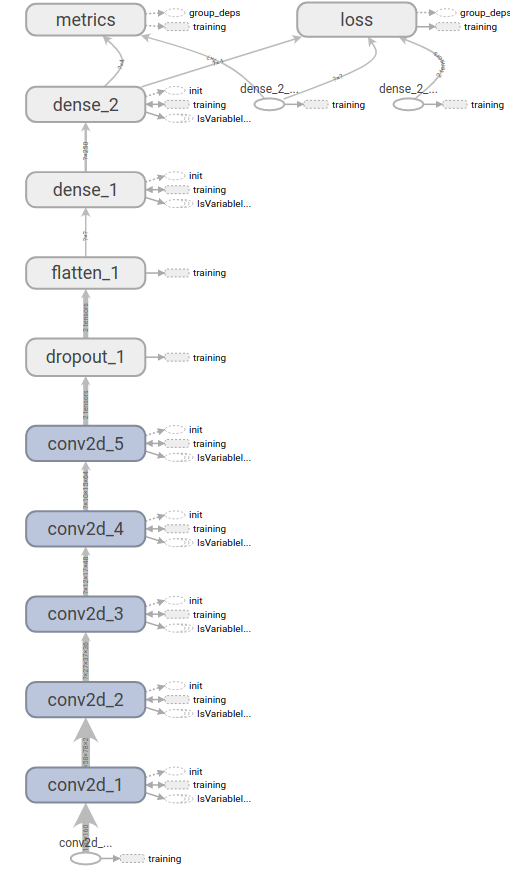
\includegraphics[width=0.5\textwidth,height=0.5\textheight]{net-structure.png}}
\caption{Model Structure.}
\label{ms}
\end{figure}

CNN layers can extract features from the images taken by the car's front camera. Some fully connected layers follow the CNN layers, they can finally extract the command information needed for auto-driving. The activation function we use is Relu. The last layer can be a Softmax layer\cite{b25} for classification or a Dense layer for regression.  

Although the current model is not the perfect one, it's convenient to make changes and do optimizations to the model.

\textbf{Computer Vision Analysis.} OpenCv\cite{b20} is a widely used library for computer vision analysis. Due to the native support for OpenCv in Pynq-Z2, users can easily invoke existing computer vision algorithms. We also provide some commonly used algorithms as follows. Theses algorithms are implemented in C++ with OpenCV. They can be very time consuming running in ARM Cortex-A9 in Xilinx PYNQ-Z2. To reduce computation complexity, we can do some pre-process like cropping and down-sampling. Some time consuming tasks such as Gaussian filter, Canny edge detection, Hough transform can be moved to FPGA using Xilinx xfopencv library\cite{b30}, BP neural network can be implemented in FPGA using Xilinx Vivado HLS. However, when implementing accelerators in FPGA, users should take the board's resource into consideration and choose the heaviest computational task to implement while not beyond the resource limit.

\begin{itemize}
\item{Road lane detection.} To detect road lane, we first use 5*5 Gaussian filter to remove the noise of the image. Then Canny edge detection\cite{b26} is applied to detect the edges of the image. Hough transform\cite{b27} is employed to detect the lines of the image. Based on the orientation and relative position of detected lines, side line and stop line of the road can be identified. 

To improve the robustness and accuracy of the algorithm, more techniques will be added to the algorithm, such as K-Means clustering\cite{b28} for Hough lines, Kalman/Gabor filtering for sampled data, alternative IPM (inverse perspective mapping) lane detection method\cite{b29}.

\item{Traffic light recognition.} To recognize the traffic light, we first use IHLS color space\cite{b31} to remove the disturbance of the color in complicated background. After obtaining the color information, Hough circle transform\cite{b32} is applied to get the shape information of the traffic light. Combing the shape and color information, traffic light or similar objects can be detected. Finally, a simple BP neural network is employed to accurately recognize the traffic light in the contest.

\end{itemize}

\textbf{DPU Acceleration. }The DPU\cite{b17} is one accelerator in FPGA, it can accelerate the process of AI reference. We provide some scripts to do a complete set of optimized tool chains provided by DNNDK, including compression, compilation and runtime. You can refer to Fig.~\ref{df} to see the framework of DNNDK. 

After using DPU, the fps can be which means it's easy for the board to perform AI reference. The model we use here is described above. 

What's more, the DPU can not only provide computation power for AI reference but users can also program the FPGA to add their own accelerators for different algorithms. So, if you are a researcher who cares mostly about hardware acceleration, you can do experiments based on our platform.

\begin{figure}[htbp]
\centerline{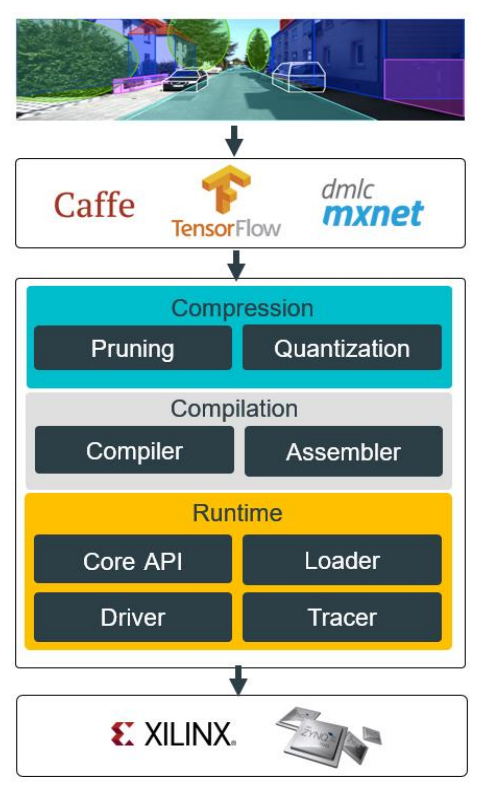
\includegraphics[width=0.5\textwidth,height=0.5\textheight]{DNNDK.PNG}}
\caption{DNNDK Framework\cite{b17}.}
\label{df}
\end{figure}

\section{Key Characteristics}
The xxx platform has three key characteristics: high flexibility and extensibility, full stack, and easy-to-use. These three characteristics can help users understand AD technology stack and the platform.

\textbf{High Flexibility and Extensibility. }The idea of our system design is inspired by ROS. In ROS, you can easily add new functions by adding ROS nodes. Nodes can easily get and send messages through the publish-subscribe mechanism. What we do is making the ROS system more lightweight and forthright. The thread is similar to node while the producer–consumer model is similar to the publish-subscribe mechanism. So it's easy to add more hardware devices as sensors or threads as handlers. What's more, due to the base of our system is Ubuntu18.04, it's easy to redefine the whole software framework as you like, actually we have an example of using ROS in following case studies.

\textbf{Full Stack. }The full stack here means our product provide almost everything you need to learn about AD technologies from algorithms to hardware. It's important for researchers or students to understand how the car runs and why sophisticated algorithms can be run in resource limited edge platform. Users can use different physical construction, different operating system, different software framework, different algorithm and different hardware acceleration etc. That means researchers can do whatever research they want based on our platform and they can easily use existing modules and understand the operation mode of the whole system. Considering the difficulty users may have in collecting training data and testing AI models in real world, we provide a simulator in Unity3d which is a game engine. Users can easily use the simulator to do some tests or more. The simulator usage will be introduced in case studies.

\textbf{Easy-to-Use. }The most important thing we believe is to make our platform easy to use. To achieve this, most libraries of the platform are familiar to users like OpenCv and TensorFlow\cite{b33}, they are open-sourced and widely used. Most importantly, the basic knowledge users should know includes only Linux, C++,Python, AI and a little about DPU usage. The software framework is simple and tidy, we only keep necessary functions and make it extendable. The hardware is simple too, if you don't want to add more devices, one camera and two motors are all you have to deal with. Users even don't have to prepare a real car to do experiments, then you can care nothing about hardware. Besides, we provide many documents for users, so it's easy for them to modify any part of the platform.

\section{Case Studies}
In this section, we use three case studies deployed on xxxx to show the capabilities of our research platform.

\subsection{Autonomous Driving with DPU power}
This case shows how you can use our platform to train an AI model and use it for autonomous driving. 

First, you can control the car using your keyboard or whatever you like and save data from the car's sensors as training data. Or you can just get the data from Internet or somewhere else. 

Second, after some pre-process, you can put the images you get as input to the AI model and the labels such as keyboard signals as the output. Train the model using TensorFlow until you get a satisfy model.

Third, you will use DNNDK\cite{b17} provided by Xilinx to do the compression and compilation and then copy the generated files to the car.

Finally, the car can move by itself. It will be controlled by AI models or other algorithms added. 

\subsection{Simulator}
The simulator is a tool which can help users test their designs more efficiently. You can see the interface of the simulator in Fig.~\ref{si}. The simulator is based on sdsandbox\cite{b5} which is a simulator project for Donkey Car\cite{b34}. As you can see in the picture, the users can use this simulator to collect training data and test their models. 
When testing, you should build a server, the server will receive sensor data from the client of the simulator and generate control messages according to these data. We have already built one example, the server will get images taken by simulator and handles them using the AI model trained before, then the model output control commands and these commands will be sent to the simulator.
It's also convenient for users to modify the source code of the simulator to define their own data format or control methods. However, users should be familiar with C\# and Unity3d if they would like to do so, and we provide some coding tutorial manual to help.

\subsection{ROS Usage}
Due to the high impact of ROS, we make our platform able to support ROS projects. The version we use is ROS Melodic\cite{b35} which is mainly used in Ubuntu18.04. 
This time we show how to read LiDAR data and control the car using ROS. With LiDAR data, the car can handle obstacle avoidance tasks and LiDAR data processing is the basic of SLAM map-building

\begin{figure}[htbp]
\centerline{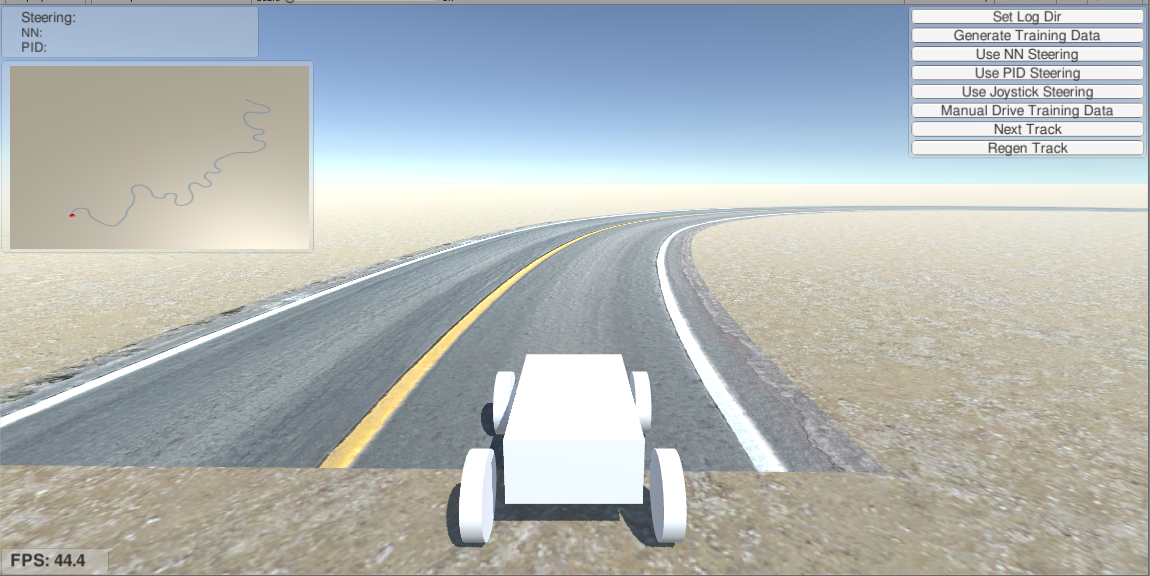
\includegraphics[width=0.5\textwidth]{simulator.png}}
\caption{Simulator Interface.}
\label{si}
\end{figure}


\begin{thebibliography}{00}

\bibitem{b1} Liu, Shaoshan, Liyun Li, Jie Tang, Shuang Wu, and Jean-Luc Gaudiot. "Creating autonomous vehicle systems." Synthesis Lectures on Computer Science 6, no. 1 (2017): i-186.

\bibitem{b2} Daniel Nurmi, Rich Wolski, Chris GrzegorczykGraziano Obertelli, Sunil Soman, Lamia Youseff, and Dmitrii Zagorodnov. The eucalyptus open-source cloud-computing system. In Cluster Computing and the Grid, 2009. CCGRID’09. 9th IEEE/ACM International Symposium on, pages 124–131. IEEE, 2009.

\bibitem{b3} Jeffrey Dean and Sanjay Ghemawat. Mapreduce: simplified data processing on large clusters. Communications
of the ACM, 51(1):107–113, 2008.

\bibitem{b4} TUL Unity3d Available at: https://unity.com/learn

\bibitem{b5} Tawn Kramer, sdsandbox [ONLINE] Available at: https://github.com/tawnkramer/sdsandbox

\bibitem{b6} TUL PYNQ-Z2 [ONLINE] Available at: http://www.tul.com.tw/ProductsPYNQ-Z2.html

\bibitem{b7} ReleaseNotes Ubuntu 18.04 [ONLINE] Available at: https://wiki.ubuntu.com/

\bibitem{b8} TUL ARM Cortex-A9 [ONLINE] Available at: https://developer.arm.com/http://www.armdesigner.com/MINI3188/?gclid=Cj0KCQjwi7DtBRCLARIsAGCJWBpdSiwajASBuoCjuPR9pprkW7iJOfAQnCIpNK\_eJhz35TM5WoY2fYIaAhYYEALw\_wcB

\bibitem{b9} Wang, Yifan, Liangkai Liu, Xingzhou Zhang, and Weisong Shi. "HydraOne: An indoor experimental research and education platform for CAVs." In 2nd {USENIX} Workshop on Hot Topics in Edge Computing (HotEdge 19). 2019.

\bibitem{b10} Junqing Wei, Jarrod M Snider, Junsung Kim, John M Dolan, Raj Rajkumar, and Bakhtiar Litkouhi. Towards a viable autonomous driving research platform. In 2013 IEEE Intelligent Vehicles Symposium (IV), pages 763–770. IEEE, 2013.

\bibitem{b11} O'Kelly, Matthew, Varundev Sukhil, Houssam Abbas, Jack Harkins, Chris Kao, Yash Vardhan Pant, Rahul Mangharam et al. "F1/10: An Open-Source Autonomous Cyber-Physical Platform." arXiv preprint arXiv:1901.08567 (2019).

\bibitem{b12} Nurvitadhi, E., Sheffield, D., Sim, J., Mishra, A., Venkatesh, G., \& Marr, D. (2016, December). Accelerating binarized neural networks: Comparison of FPGA, CPU, GPU, and ASIC. In 2016 International Conference on Field-Programmable Technology (FPT) (pp. 77-84). IEEE.

\bibitem{b13} cuDNN Documentation [ONLINE] Available at: https://docs.nvidia.com/deeplearning/sdk/index.html\#training

\bibitem{b14} TensorRT Documentation [ONLINE] Available at: https://docs.nvidia.com/deeplearning/sdk/index.html\#inference

\bibitem{b15} TechRadar. Google's Tensor Processing Unit explained: this is what the future of computing looks like. Retrieved 2017-01-19. [ONLINE] Available at: https://www.techradar.com/news/computing-components/processors/google-s-tensor-processing-unit-explained-this-is-what-the-future-of-computing-looks-like-1326915

\bibitem{b16} Tensor\_processing\_unit, Wikipedia [ONLINE] Available at: https://en.wikipedia.org/wiki/Tensor\_processing\_unit

\bibitem{b17} TUL DNNDK [ONLINE] Available at: https://www.xilinx.com/support/documentation/sw\_manuals/ai\_inference /v1\_5

\bibitem{b18} Producer–consumer problem, Wikipedia [ONLINE] Available at: https://en.wikipedia.org/wiki/Producer\_consumer\_problem

\bibitem{b19} Morgan Quigley, Ken Conley, Brian Gerkey, Josh Faust, Tully Foote, Jeremy Leibs, Rob Wheeler, and Andrew Y Ng. ROS: An open-source robot operating system. In ICRA workshop on open source software, page 5. Kobe, Japan, 2009.

\bibitem{b20} OpenCv [ONLINE] Available at: https://opencv.org/

\bibitem{b21} Bojarski, M., Testa, D. D., Dworakowski, D., Firner, B., Flepp, B., Goyal, P., Jackel, L. D., Monfort, M., Muller, U., Zhang, J., Zhang, X., Zhao, J., and Zieba, K. End to end learning for self-driving cars. CoRR abs/1604.07316 (2016)

\bibitem{b22} Chi, L., and Mu, Y. Deep steering: Learning end-to-end driving model from spatial and temporal visual cues. arXiv preprint arXiv:1708.03798 (2017).

\bibitem{b23} Eraqi, H. M., Moustafa, M. N., and Honer, J. End-to-end deep learning for steering autonomous vehicles considering temporal dependencies. arXiv preprint arXiv:1710.03804 (2017)

\bibitem{b24} Kendall, A., Hawke, J., Janz, D., Mazur, P., Reda, D., Allen, J.-M., Lam, V.-D., Bewley, A., and Shah, A. Learning to drive in a day. arXiv preprint arXiv:1807.00412 (2018)

\bibitem{b25} Keras Documentation [ONLINE] Available at: https://keras.io/layers/core/

\bibitem{b26} John Canny, "A Computational Approach to Edge Detection, "IEEE Transactions on Pattern Analysis and Machine Intelligence, pp.679-698, 1986.

\bibitem{b27} J. B. Burns, A. R. Hanson and E. M. Riseman, "Extracting Straight Lines," in IEEE Transactions on Pattern Analysis and Machine Intelligence, vol. PAMI-8, no. 4, pp. 425-455, July 1986.

\bibitem{b28} S. Selim, M. Ismail, "K-Means-Type Algorithms: A Generalized Convergence Theorem and Characterization of Local Optimality," Pattern Analysis and Machine Intelligence, IEEE Transactions on, vol. 6, no. 1, pp. 81-87, 1984. 

\bibitem{b29} Jun Wang, Tao Mei, Bin Kong and Hu Wei, "An approach of lane detection based on Inverse Perspective Mapping," 17th International IEEE Conference on Intelligent Transportation Systems (ITSC), Qingdao, 2014, pp. 35-38.

\bibitem{b30} Xilinx. (2019, Sep) Xilinx/xfopencv. [ONLINE]. Available:  https://github.com/Xilinx/xfopencv

\bibitem{b31} Allan Hanbury and Jean Serra, "A 3d-polar coordinate colour representation well adapted to image analysis," in Proceedings of the Scandinavian Conference on Image Analysis (SCIA), 2003, pp. 804–811.

\bibitem{b32} M. Rizon et al., 2005, "Object Detection using Circular Hough Transform", American Journal of Applied Sciences 2, vol 12, pp. 1606-1609.

\bibitem{b33} TensorFlow [ONLINE] Available at: https://www.tensorflow.org

\bibitem{b34} Donkey Car [ONLINE] Available at: https://www.donkeycar.com
\end{thebibliography}

\bibitem{b35} ROS Melodic [ONLINE] Available at: http://wiki.ros.org/melodic/
\vspace{12pt}

\end{document}
